% SLIDE 1: pagina di presentazione
\frame{\titlepage}

% SLIDE 2: motivazioni
\begin{frame}
    \frametitle{Scenario e Motivazioni}
    Il mondo del Cloud ha portato molti benefici, tuttavia solleva diverse problematiche legate alla \alert{mancanza di fiducia}
    \hfill\break
    \begin{itemize}
        \item Non vengono fornite agli utenti le specifiche riguardanti le misure di sicurezza messe in atto
        \item Sono sistemi specifici e \alert{difficili da utilizzare} se non si ha esperienza in materia
    \end{itemize}
\end{frame}

% SLIDE 3: motivazioni
\begin{frame}
    \frametitle{Scenario e Motivazioni (2)}
    \begin{columns}
        \begin{column}{0.55\textwidth}
            Moon Cloud è una piattaforma erogata come servizio, la quale supporta:
            \begin{itemize}
                \item un sistema di \textit{Security Governance}
                \item un framework di \alert{\textit{Security Assurance}}
            \end{itemize}
        \end{column}
        \begin{column}{0.4\textwidth}
            \begin{center}
                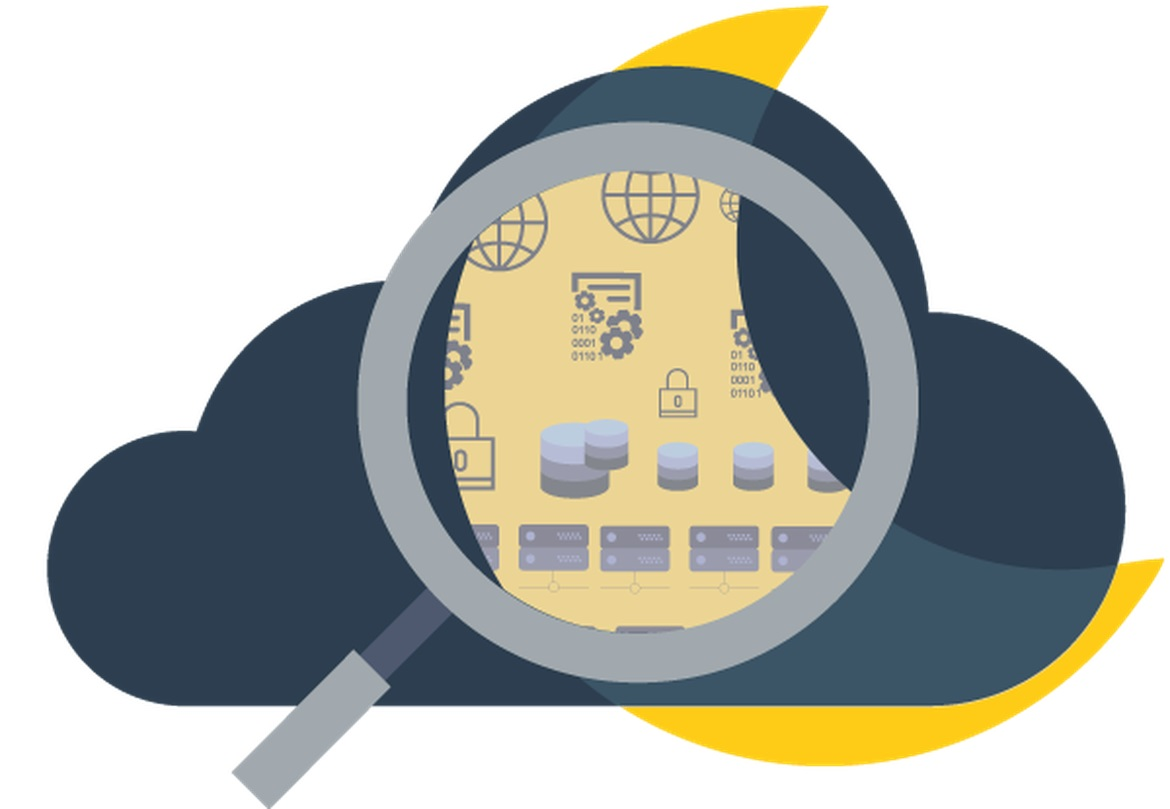
\includegraphics[scale=0.12]{images_pres/mc}
            \end{center}
        \end{column}
    \end{columns}
    Garantisce il controllo della sicurezza informatica in modo rapido ed efficiente, attraverso attività di test e monitoraggio 
    periodiche e programmate
\end{frame}

% SLIDE 4: obiettivi
\begin{frame}
    \frametitle{Obiettivo della tesi}
    Introdurre un \alert{sistema di raccomandazione} che possa consigliare all'utente delle possibili \textit{Evaluation} rispetto 
    al \textit{target} indicato da proteggere e monitorare
    \begin{itemize}
        \item L'utente meno esperto può usufruire dei servizi offerti da Moon Cloud in modo \alert{semplice} e \alert{intuitivo}
        \item Si è cercato di colmare il problema della mancata fiducia in questi sistemi
    \end{itemize}

\end{frame}

% SLIDE 5:
\begin{frame}
    \frametitle{Sistema di raccomandazione}

\end{frame}

% SLIDE 5:
%\begin{frame}
%    \frametitle{}

%\end{frame}

% SLIDE 6:
%\begin{frame}
%    \frametitle{}

%\end{frame}

% SLIDE 7:
%\begin{frame}
%    \frametitle{}

%\end{frame}

% SLIDE 8:
%\begin{frame}
%    \frametitle{}

%\end{frame}

% SLIDE 9:
%\begin{frame}
%    \frametitle{}

%\end{frame}

% SLIDE 10:
%\begin{frame}
%    \frametitle{}

%\end{frame}

% SLIDE 11:
%\begin{frame}
%    \frametitle{}

%\end{frame}

% SLIDE 12:
%\begin{frame}
%    \frametitle{}

%\end{frame}